
\documentclass{statsoc}
\usepackage{graphicx}
\usepackage{listings}
\usepackage{color}
\usepackage{amssymb, amsmath, geometry}
\usepackage{natbib}
\usepackage{hyperref}

\makeatletter
\def\maxwidth{\ifdim\Gin@nat@width>\linewidth\linewidth\else\Gin@nat@width\fi}
\def\maxheight{\ifdim\Gin@nat@height>\textheight\textheight\else\Gin@nat@height\fi}
\makeatother
% Scale images if necessary, so that they will not overflow the page
% margins by default, and it is still possible to overwrite the defaults
% using explicit options in \includegraphics[width, height, ...]{}
\setkeys{Gin}{width=\maxwidth,height=\maxheight,keepaspectratio}

\title[Forecasting brazilian inflation using ARIMA and ETS
models]{Forecasting brazilian consumer price index monthly variation
using ARIMA and ETS models}




 
\author[William Edward Rappel de Amorim]{William Edward Rappel de
Amorim}
\address{University of Brasilia,
Brasilia-DF,
Brazil}
\email{william\_rappel@hotmail.com}



% BIBLIOGRAPHY
\usepackage[authoryear]{natbib}
\bibpunct{(}{)}{;}{a}{}{,}


% tightlist command for lists without linebreak
\providecommand{\tightlist}{%
  \setlength{\itemsep}{0pt}\setlength{\parskip}{0pt}}



\usepackage{booktabs}
\usepackage{longtable}
\usepackage{array}
\usepackage{multirow}
\usepackage{wrapfig}
\usepackage{float}
\usepackage{colortbl}
\usepackage{pdflscape}
\usepackage{tabu}
\usepackage{threeparttable}
\usepackage{threeparttablex}
\usepackage[normalem]{ulem}
\usepackage{makecell}
\usepackage{xcolor}

\begin{document}


\begin{abstract}
Inflation forecasting is an extremely important task, as it can help
economic agents make decisions. The aim of this study was to use ARIMA
and ETS models to forecast monthly variation in the IPCA, the main
inflation index used in Brazil. The ARIMA model presented residuals with
satisfactory behavior, whereas the ETS presented non-independence.
However, both showed very low predictive performance.
\end{abstract}
\keywords{Time series, Forecasting, Time series forecasting, State Space
Models, Inflation, IPCA, CPI, ARIMA, ETS, Statistics, Predictive
modelling.}

\hypertarget{introduction}{%
\section{Introduction}\label{introduction}}

The Brazilian consumer price index, known in Brazil as the IPCA, is the
most widely used index to measure economic inflation for the Brazilian
consumer. It is used as a readjustment indicator for several contracts
and is an important economic indicator, with a great impact on the
decision-making process of economic agents, both public and private.
Thus, making accurate predictions of this indicator is extremely
important for better planning and defining each agent's strategy.

In this article, the object of study was the time series of the monthly
variation of the IPCA, presented by the Central Bank of Brazil,
available at
\url{https://www3.bcb.gov.br/sgspub/localizarseries/localizarSeries.do?method=prepararTelaLocalizarSeries}.
It was decided to use only the last 15 years of this series, that is,
starting in January 2008. Then, ARIMA and ETS models were estimated.
After that, it was conducted residual analysis, followed by an study of
the predictive performance via sliding window technique. Finally, point
and interval predictions were obtained and evaluated in a test set.

The series has a monthly frequency and 15 years of observations,
totaling 180 values. It was divided into train and test datasets, with
the training period from 2008 to 2021 and the testing period is the year
of 2022. Figure 1 presents the observed values of the time series in the
training period. It appears to be stationary, but the mean of the series
is greater than 0.

\begin{figure}

{\centering 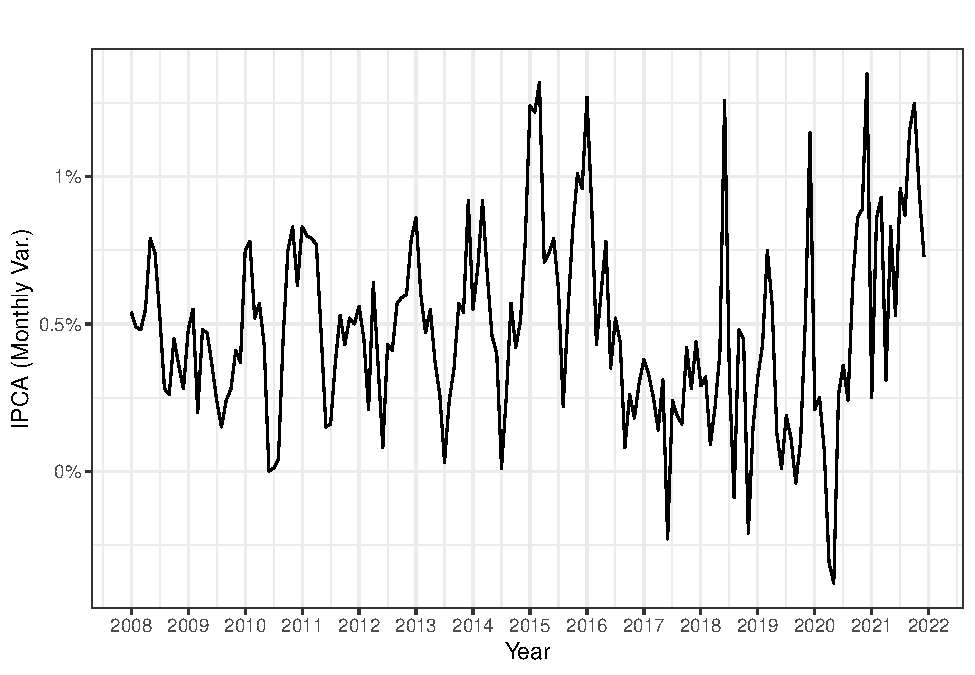
\includegraphics[height=0.4\textheight]{Trabalho_2_article_files/figure-latex/ipca-plot-1} 

}

\caption{Monthly variation of the IPCA.}\label{fig:ipca-plot}
\end{figure}

\hypertarget{decomposition}{%
\section{Decomposition}\label{decomposition}}

The STL decomposition was applied to the training series, via
\texttt{mstl} function from the \texttt{forecast} R package. This R
package was proposed by \citet{forecast}. Results are shown in Figure 2.
It is not possible to identify a very intense trend or seasonal pattern.

\begin{figure}

{\centering 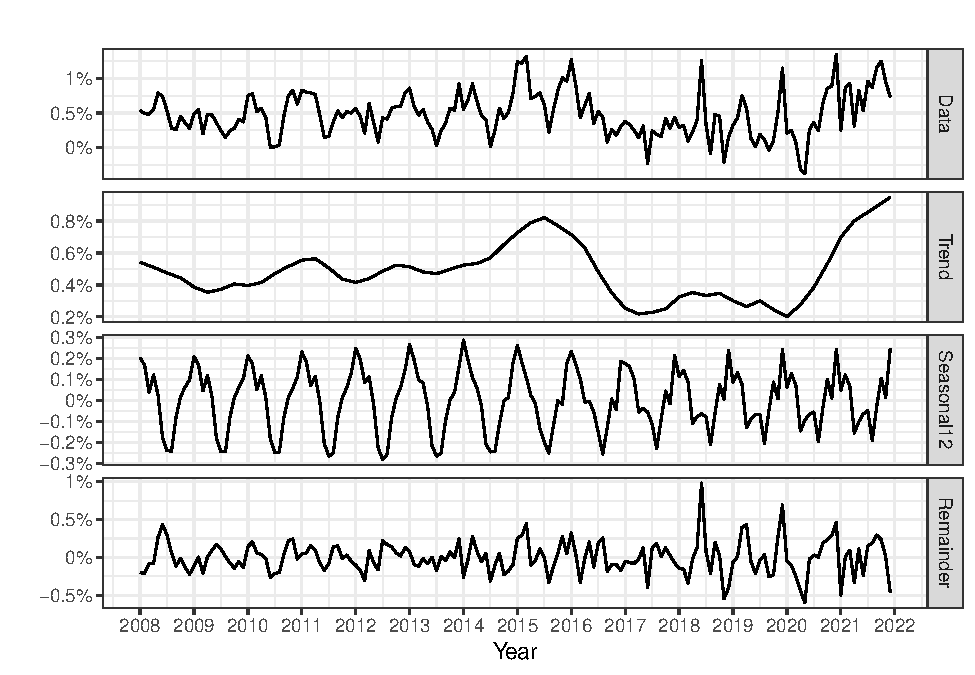
\includegraphics[height=0.4\textheight]{Trabalho_2_article_files/figure-latex/mstl-1} 

}

\caption{STL decomposition of the training series.}\label{fig:mstl}
\end{figure}

\hypertarget{model-selection}{%
\section{Model selection}\label{model-selection}}

In this article, the ARIMA and ETS model classes were considered. In
addition, Box-Cox transformations were not used, since the level of
variation in the series appears to be constant.

\hypertarget{arima}{%
\subsection{ARIMA}\label{arima}}

ARIMA models are described at \citet{morettin2006}. Via \texttt{ndiffs}
and \texttt{nsdiffs} function from the \texttt{forecast} R package, it
is obtained that differentiations are not necessary, as the series is
already stationary (Figure 1), a hypothesis confirmed by the Augmented
Dickey Fuller test (p-value = 0.01). From Figure 1, it can be seen that
the mean of the series is greater than 0, a fact that will be considered
in the training of the ARIMA models. Next, in order to select the
parameters \(p\), \(q\), \(P\) and \(Q\), the ACF and PACF are presented
in Figure 3.

\begin{figure}

{\centering 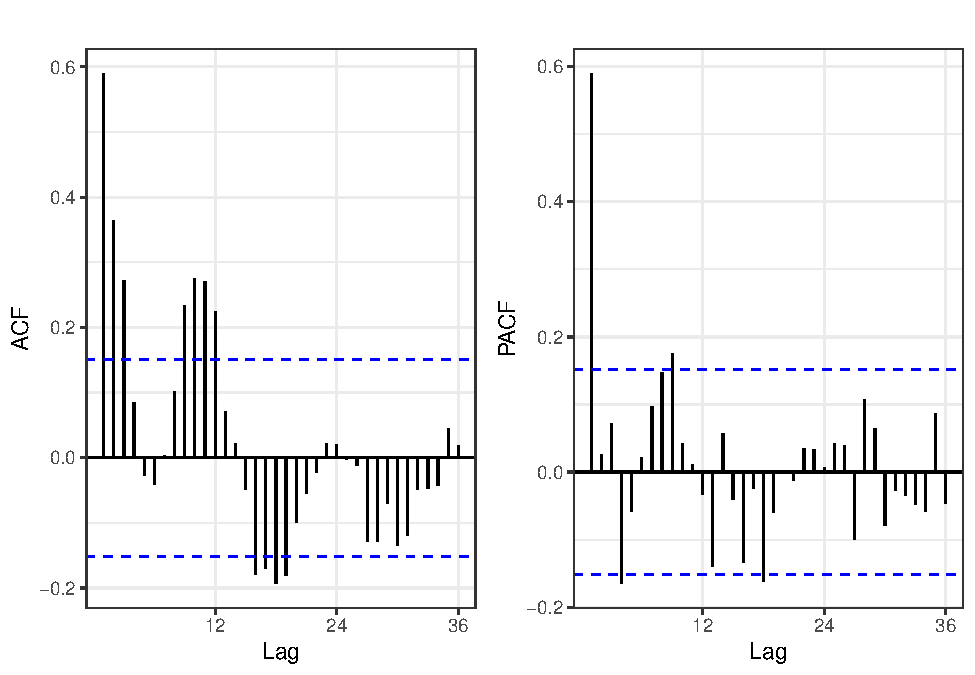
\includegraphics[height=0.4\textheight]{Trabalho_2_article_files/figure-latex/acf-pacf-1} 

}

\caption{ACF and PACF plots.}\label{fig:acf-pacf}
\end{figure}

When analyzing the non-seasonal lags, the ACF converges to zero without
breaks, while the PACF shows a break in the first lag. Therefore, the
chosen candidate values are \(p\) equals 1 and \(q\) equals 0. For
seasonal lags, the PACF is not significantly different from 0 at any lag
and the ACF is significant only at lag 12. So \(P\) will be fixed at 0
and \(Q=0,1\). After training ARIMA models with all the combinations of
parameters described earlier, the model with the lowest AICc is
selected, which is the \(SARIMA(1,0,0)(0,0,1)_{12}\) and AICc equals to
31.62.

\begin{figure}

{\centering 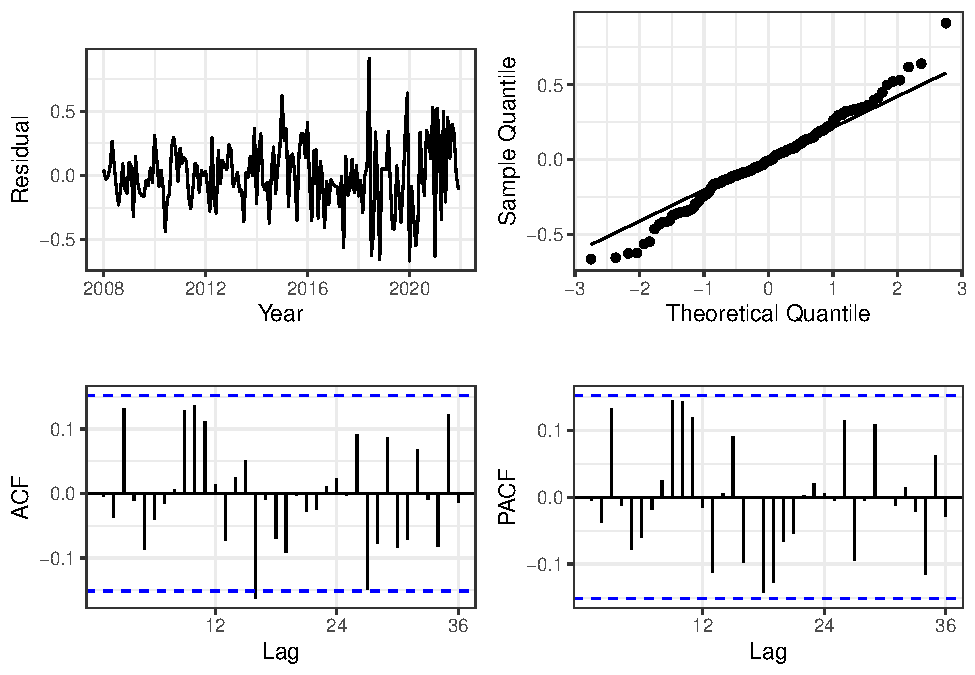
\includegraphics[height=0.4\textheight]{Trabalho_2_article_files/figure-latex/arima-residuals-plots-1} 

}

\caption{ARIMA residuals plots.}\label{fig:arima-residuals-plots}
\end{figure}

From Figure 4 and Shapiro-Wilk and Ljung-Box tests, it is concluded that
the residuals appear to be stationary, normally distributed (p-value =
0.18) and independent (p-value = 0.39).

\hypertarget{ets}{%
\subsection{ETS}\label{ets}}

ETS models are described at \citet{hyndman2008}. As the series does not
have a seasonal pattern, only ETS models without a seasonal component
will be considered. The best model will be defined using the
\texttt{ets} function from the \texttt{forecast} R package, which trains
several ETS models and selects the one with the lowest value for the
AICc. After applying this procedure, the model selected is ETS(A,N,N),
which corresponds to the SES model and has AICc equals to 440.21.

\begin{figure}

{\centering 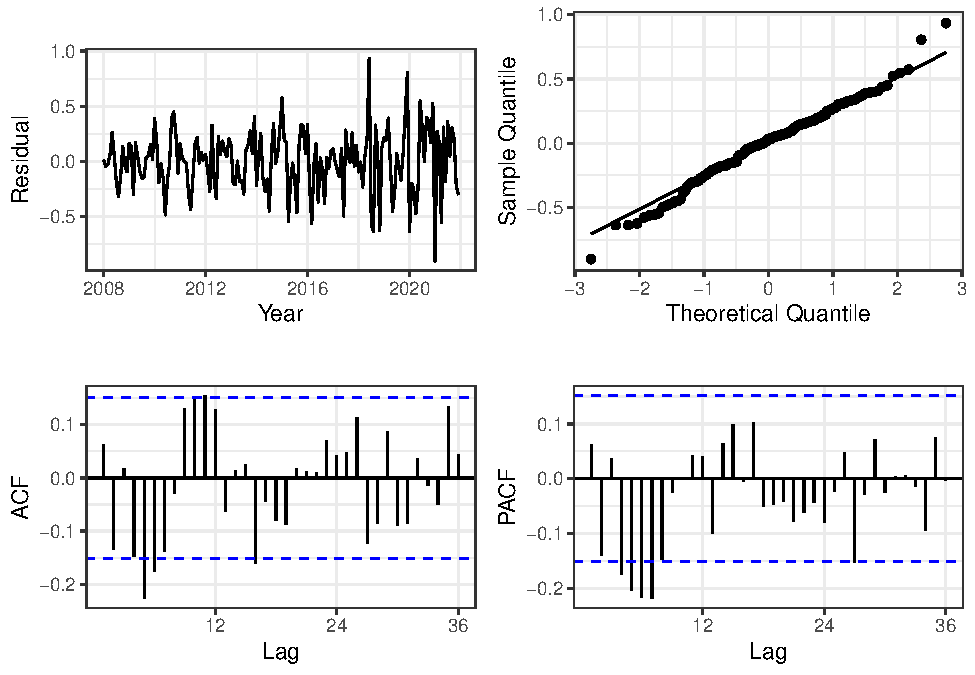
\includegraphics[height=0.4\textheight]{Trabalho_2_article_files/figure-latex/ets-residuals-plots-1} 

}

\caption{ETS residuals plots.}\label{fig:ets-residuals-plots}
\end{figure}

From Figure 5 and Shapiro-Wilk and Ljung-Box tests, it is concluded that
the residuals appear to be stationary, normally distributed (p-value =
0.14), but not independent (p-value \textless{} 0.01).

\hypertarget{predictive-performance-analysis}{%
\section{Predictive performance
analysis}\label{predictive-performance-analysis}}

Using only the training dataset, the predictive performance of the
selected ARIMA and ETS models was evaluated via sliding window, starting
at the 13th month of observation and considering predictions of up to 12
steps ahead.

\begin{table}

\caption{\label{tab:sliding-window-table}MAE by horizon.}
\centering
\begin{tabular}[t]{lcc}
\toprule
  & ARIMA & ETS\\
\midrule
h=1 & 0.207 & 0.230\\
h=2 & 0.239 & 0.281\\
h=3 & 0.246 & 0.314\\
h=4 & 0.256 & 0.346\\
h=5 & 0.262 & 0.351\\
\addlinespace
h=6 & 0.266 & 0.363\\
h=7 & 0.264 & 0.345\\
h=8 & 0.263 & 0.329\\
h=9 & 0.262 & 0.297\\
h=10 & 0.264 & 0.295\\
\addlinespace
h=11 & 0.267 & 0.307\\
h=12 & 0.270 & 0.308\\
\bottomrule
\end{tabular}
\end{table}

\begin{figure}

{\centering 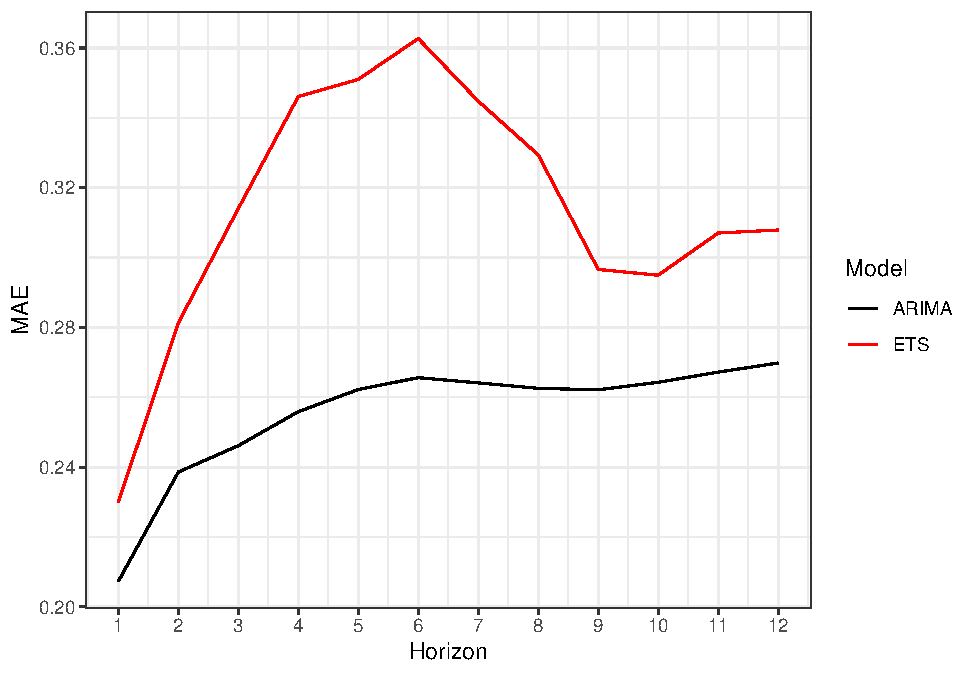
\includegraphics[height=0.4\textheight]{Trabalho_2_article_files/figure-latex/sliding-window-plot-1} 

}

\caption{MAE by forecasting horizon.}\label{fig:sliding-window-plot}
\end{figure}

From Figure 6, the most accurate model in all forecasting horizons
considered is ARIMA. Then, point predictions for the test dataset were
obtained using these 2 models and 9 more benchmarks available in the
forecast package: \texttt{naive}, \texttt{meanf}, \texttt{holt},
\texttt{hw}, \texttt{auto.arima}, \texttt{stlf}, \texttt{bats},
\texttt{tbats}, \texttt{thetaf}. In Table 2, the MAEs of each of the
considered models are presented.

\begin{table}

\caption{\label{tab:benchmark}MAE on test.}
\centering
\begin{tabular}[t]{lc}
\toprule
  & MAE\\
\midrule
ARIMA & 0.162\\
ETS & 0.365\\
naive & 0.262\\
meanf & 0.128\\
holt & 0.379\\
\addlinespace
hw & 0.385\\
auto.arima & 0.162\\
sltf & 0.317\\
bats & 0.307\\
tbats & 0.358\\
\addlinespace
thetaf & 0.434\\
\bottomrule
\end{tabular}
\end{table}

Thus, the \texttt{meanf} benchmark, which uses the historical average as
a point forecast, was the one that obtained the lowest MAE among all
models considered. In Figure 7, point and interval forecasts are
presented considering this model.

\begin{figure}

{\centering 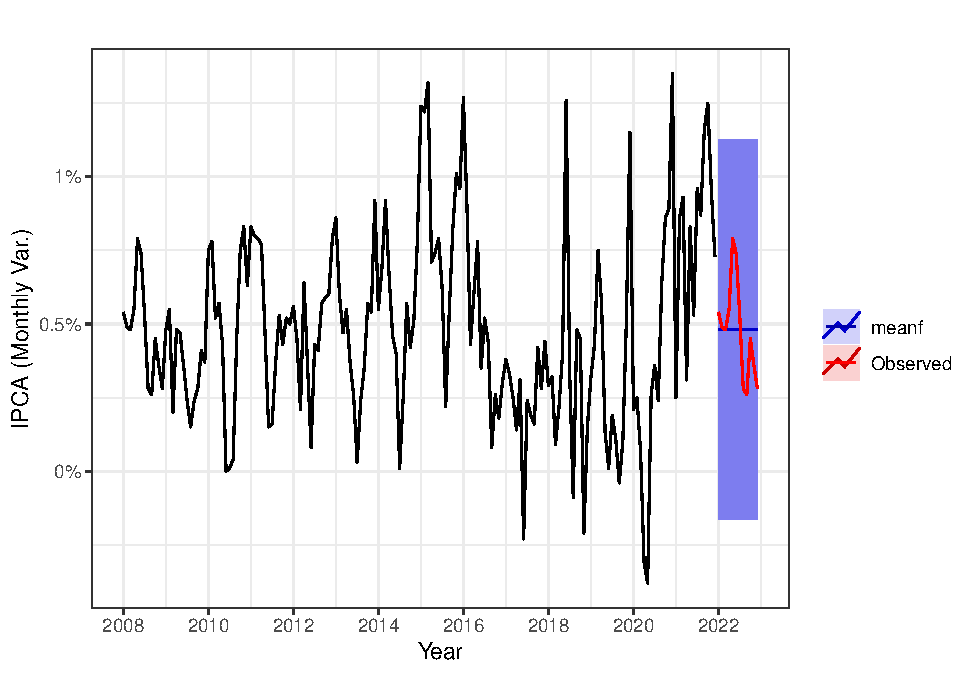
\includegraphics[height=0.4\textheight]{Trabalho_2_article_files/figure-latex/preds-plot-1} 

}

\caption{Point and interval prediction using meanf.}\label{fig:preds-plot}
\end{figure}

\hypertarget{conclusion}{%
\section{Conclusion}\label{conclusion}}

In this article, after adjusting the ARIMA model to the IPCA monthly
variation series, the residuals presented all the desired
characteristics. As for the ETS model, the residuals are not
independent. However, both models have very low predictive performance,
being surpassed by the simple benchmark of the historical average. Other
studies are needed to increase the predictive performance through the
inclusion of explanatory variables and adjustments of dynamic regression
models.

\bibliographystyle{rss}
\bibliography{bibliography}


\end{document}
